\subsection{tt.go} 

The main structure in "tt.go" is typetable. It contains information for mapping a concrete type to its hash using a "*trie" data structure for hash to type and a "map[reflect.Type]types.Hash" for type to hash information. Detailed information of "*trie" and "types.Hash" are in "trie.go" and "types.go".

The constructor for typetable is:

\begin{itemize}

	\item \emph{func newTypeTable() *typetable}\\
	Returns a new typetable structure with an empty *trie and map[reflect.Type]types.Hash.
	
\end{itemize}

Exported methods of typetable:

\begin{itemize}

	\item \emph{func (*typetable) Register(reflect.Type, types.Hash) bool}\\
	Maps the concrete type of the value contained in the empty interface to its hash and stores it into the *trie and map[reflect.Type]types.Hash data structures.
	
	\item \emph{func (*typetable) TypeForHash(types.Hash) reflect.Type}\\
	Given an hash returns the corresponding type.
	
	\item \emph{(*typetable) HashForType(reflect.Type) types.Hash}\\
	Given a type returns the corresponding hash value.
	
\end{itemize}

\begin{figure}[H]
\centering
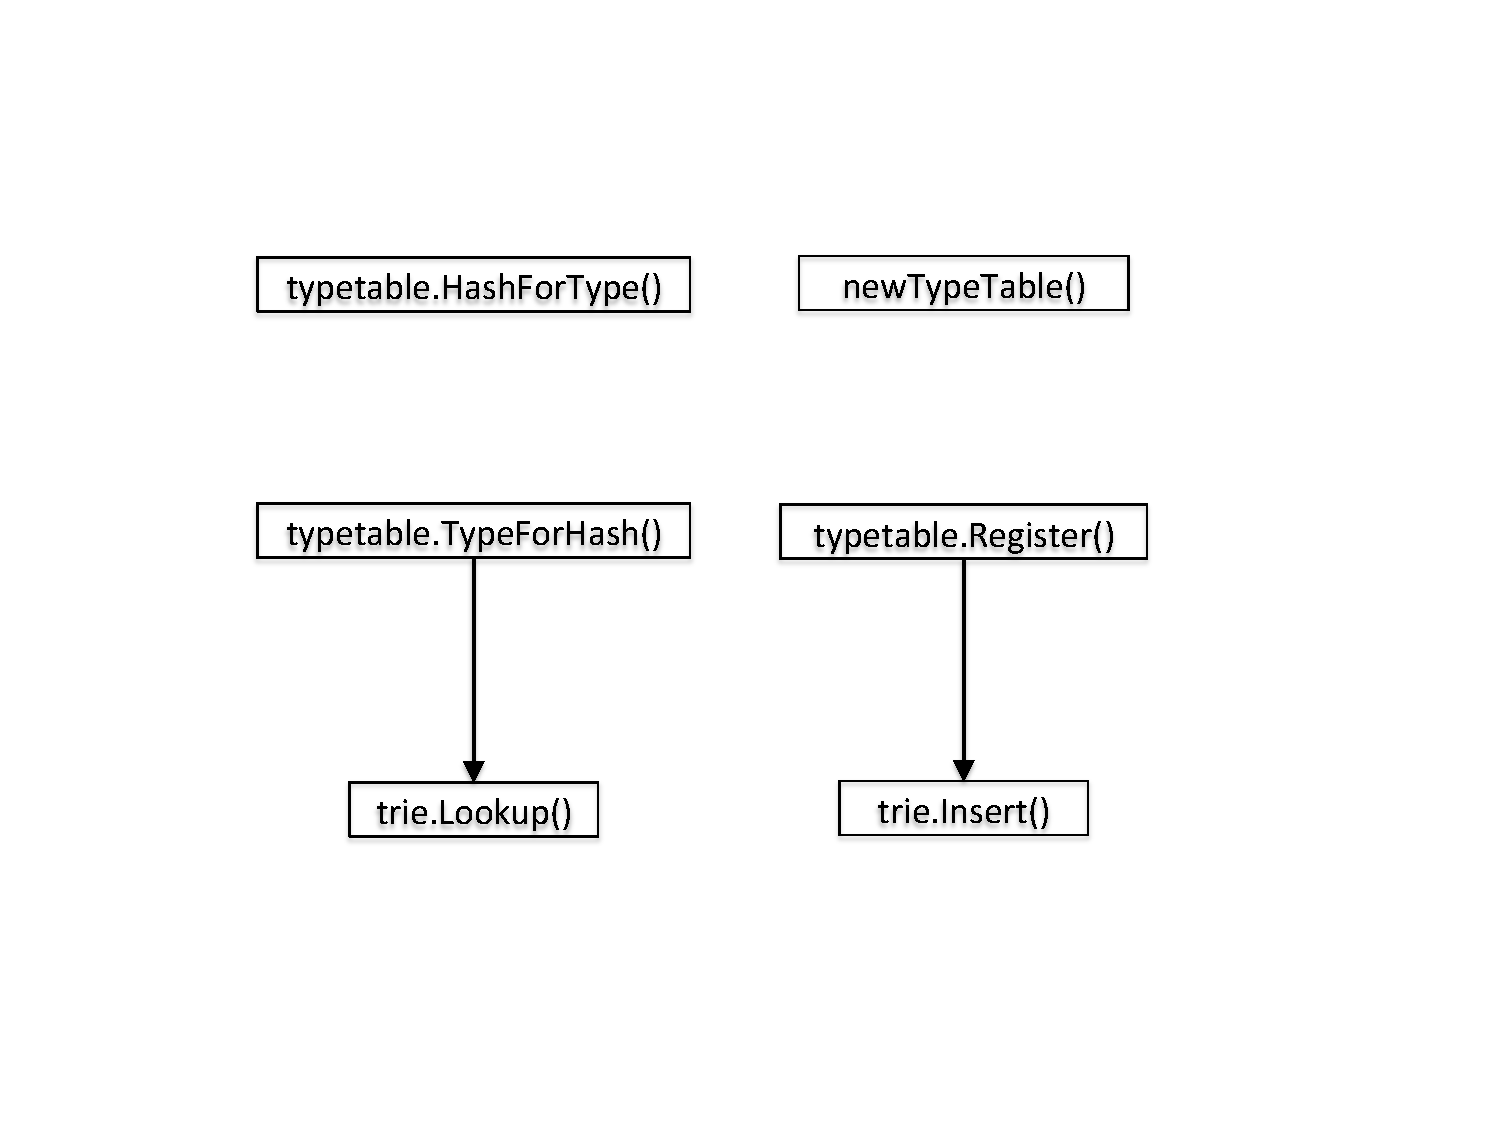
\includegraphics[scale=0.50]{callGraphs/ttPackage}
\caption{tt.go package}
\end{figure}